\documentclass[11pt,a4paper]{article}

\usepackage[utf8]{inputenc}
\usepackage[T1]{fontenc}
\usepackage{lmodern}
\usepackage[margin=0.74in]{geometry}
\usepackage[table]{xcolor}
\usepackage{array}
\usepackage{tabularx}
\usepackage{booktabs}
\usepackage{enumitem}
\usepackage{titlesec}
\usepackage{fancyhdr}
\usepackage{lastpage}
\usepackage{hyperref}
\usepackage{tikz}
\usepackage{pgfplots}

\pgfplotsset{compat=1.18}
\usetikzlibrary{arrows.meta}

\definecolor{TextInk}{HTML}{222222}
\definecolor{HeadingInk}{HTML}{333333}
\definecolor{AsiaBlue}{HTML}{1D5961}
\definecolor{AfricaRed}{HTML}{B94838}
\definecolor{RuleGray}{HTML}{D5D5D5}
\definecolor{SoftGray}{HTML}{F2F2F2}
\definecolor{EfficientGray}{HTML}{B7B7B7}

\hypersetup{
  colorlinks=true,
  linkcolor=HeadingInk,
  urlcolor=AsiaBlue,
  pdftitle={IB Geography SL Paper 1 Full Simulation Set 1 - 2026-05-07},
  pdfauthor={IB Geography SL Preparation}
}

\color{TextInk}
\setlength{\parskip}{0.48em}
\setlength{\parindent}{0pt}
\setlength{\tabcolsep}{5pt}
\renewcommand{\arraystretch}{1.18}
\setlist[enumerate]{leftmargin=1.7em,itemsep=0.8em,topsep=0.45em}
\setlist[itemize]{leftmargin=1.3em,itemsep=0.3em,topsep=0.2em}

\newcolumntype{Y}{>{\raggedright\arraybackslash}X}
\newcolumntype{L}[1]{>{\raggedright\arraybackslash}p{#1}}
\newcolumntype{C}[1]{>{\centering\arraybackslash}p{#1}}

\titleformat{\section}
  {\normalfont\Large\sffamily\bfseries\color{HeadingInk}}
  {}{0pt}{}
\titleformat{\subsection}
  {\normalfont\large\sffamily\bfseries\color{HeadingInk}}
  {}{0pt}{}

\pagestyle{fancy}
\setlength{\headheight}{14pt}
\fancyhf{}
\fancyhead[L]{\sffamily Set 1 Question Paper}
\fancyhead[R]{\sffamily IB Geography SL}
\fancyfoot[C]{\sffamily\thepage\ of \pageref{LastPage}}
\renewcommand{\headrulewidth}{0.4pt}

\newcommand{\markpts}[1]{\hfill\textbf{[#1]}}
\newcommand{\sourcepage}[2]{%
  \begin{center}
    {\sffamily\small -- #1 -- \hfill #2}
  \end{center}
}
\newcommand{\popbar}[3]{%
\begin{tikzpicture}[x=0.125cm,y=0.28cm,baseline=-0.55ex]
  \draw[RuleGray] (4,0) -- (32,0);
  \foreach \x in {4,8,12,16,20,24,28,32} {
    \draw[RuleGray] (\x,-0.2) -- (\x,0.2);
  }
  \draw[#3,line width=1.4pt,-{Latex[length=1.8mm]}] (#1,0) -- (#2,0);
\end{tikzpicture}}

\begin{document}


\newpage

\sourcepage{10}{2223--5201}

\section*{Option F -- Food and health}

Answer the following question.

\textbf{11.}\quad The simplified logarithmic graph shows the energy inputs and
outputs for different farm products in gigajoules per hectare per year.

{\sffamily\small\textbf{Key:} $\circ$ Hand cultivated \quad
$\times$ Mechanized \quad
\tikz{\draw[fill=EfficientGray,draw=black] (0,0) rectangle (0.35,0.22);}
Efficient \quad
\tikz{\draw[fill=white,draw=black] (0,0) rectangle (0.35,0.22);}
Inefficient}

\begin{center}
\begin{tikzpicture}
\begin{axis}[
  width=0.84\textwidth,
  height=0.42\textheight,
  xmode=log,
  ymode=log,
  xmin=0.05,
  xmax=200,
  ymin=0.5,
  ymax=250,
  xtick={0.05,0.1,0.2,0.5,1,2,5,10,20,50,100,200},
  xticklabels={0.05,0.1,0.2,0.5,1,2,5,10,20,50,100,200},
  ytick={0.5,1,2,5,10,20,50,100,200},
  yticklabels={0.5,1,2,5,10,20,50,100,200},
  xlabel={Energy input (gigajoules)},
  ylabel={Energy output (gigajoules)},
  axis lines=left,
  tick style={black},
  grid=none,
  clip=false,
]
  \addplot[draw=none,fill=EfficientGray] coordinates
    {(0.05,0.5) (0.05,250) (200,250) (200,200) (0.5,0.5)} -- cycle;
  \addplot[black,dashed,line width=0.8pt] coordinates {(0.5,0.5) (200,200)};
  \node[rotate=45,anchor=south,font=\sffamily\small] at (axis cs:2.1,1.35)
    {Energy efficiency ratio = 1};

  \addplot[only marks,mark=o,mark size=2.2pt,black] coordinates
    {(7,200) (0.45,55) (1.7,30)};

  \addplot[only marks,mark=x,mark size=3pt,black] coordinates
    {(25,110) (12.5,9) (50,5) (150,0.8)};

  \node[anchor=west,font=\sffamily] at (axis cs:7.5,172) {Rice};
  \node[anchor=east,font=\sffamily] at (axis cs:0.42,43) {Cassava};
  \node[anchor=east,font=\sffamily] at (axis cs:1.6,23) {Lucerne};
  \node[anchor=east,font=\sffamily] at (axis cs:24,76) {Corn};
  \node[anchor=west,font=\sffamily] at (axis cs:12.5,8.75) {Milk};
  \node[anchor=west,font=\sffamily] at (axis cs:46,4.0) {Chickens};
  \node[anchor=west,font=\sffamily] at (axis cs:150,0.7) {Lettuces};
\end{axis}
\end{tikzpicture}
\end{center}

\begin{enumerate}[label=(\alph*),leftmargin=2.2em,itemsep=0.35em,topsep=0.25em]
  \item
  \begin{enumerate}[label=(\roman*),leftmargin=2.8em,itemsep=0.2em,topsep=0.15em]
    \item Identify the farm product that has the lowest energy output.
    \markpts{1}

    \item Identify the farm product that has the highest energy efficiency.
    \markpts{1}
  \end{enumerate}

  \item Outline one way in which energy input changes as a result of
  mechanization. \markpts{2}

  \item Explain how food insecurity could be reduced by the use of:
  \begin{enumerate}[label=(\roman*),leftmargin=2.8em,itemsep=0.2em,topsep=0.15em]
    \item \emph{in vitro} meat; \markpts{3}

    \item vertical farming. \markpts{3}
  \end{enumerate}
\end{enumerate}

\textbf{(Option F continues on the following page)}

\newpage

\sourcepage{11}{2223--5201}

\textbf{(Option F continued)}

Answer either part (a) or part (b).

\textbf{Either}

\textbf{12.}\quad \textbf{(a)}\quad To what extent are diseases linked to
malnutrition? \markpts{10}

\textbf{Or}

\textbf{12.}\quad \textbf{(b)}\quad Examine how geographic factors affect the
rate of diffusion of agricultural innovation. \markpts{10}

\vfill

\begin{center}
  {\sffamily\bfseries\Large End of Option F}
\end{center}

\sourcepage{5}{2223--5201}

\section*{Option G -- Urban environments}

\textbf{13.}\quad The graph shows the ten fastest growing cities in the world
(2015--2020) and the number of new people added to each city per hour in 2020.

{\sffamily\textbf{Key:}} \textcolor{AfricaRed}{Africa};
\textcolor{AsiaBlue}{Asia}. Population arrows run from 2015 to 2020.
The final column gives new people per hour in 2020.

\rowcolors{2}{SoftGray}{white}
\begin{tabularx}{\textwidth}{C{0.07\textwidth}L{0.11\textwidth}Y C{0.33\textwidth}C{0.14\textwidth}}
\toprule
\textbf{Rank} & \textbf{Region} & \textbf{City} &
\textbf{Population (millions), 2015--2020} &
\textbf{New people per hour in 2020} \\
\midrule
1 & \textcolor{AsiaBlue}{Asia} & Delhi (India) &
\popbar{26.4}{30.9}{AsiaBlue} & 101 \\
2 & \textcolor{AsiaBlue}{Asia} & Shanghai (China) &
\popbar{24.1}{27.6}{AsiaBlue} & 82 \\
3 & \textcolor{AsiaBlue}{Asia} & Dhaka (Bangladesh) &
\popbar{18.3}{21.5}{AsiaBlue} & 76 \\
4 & \textcolor{AfricaRed}{Africa} & Kinshasa (DRC) &
\popbar{12.4}{16.2}{AfricaRed} & 75 \\
5 & \textcolor{AsiaBlue}{Asia} & Chongqing (China) &
\popbar{14.2}{16.2}{AsiaBlue} & 65 \\
6 & \textcolor{AsiaBlue}{Asia} & Lahore (Pakistan) &
\popbar{11.2}{13.4}{AsiaBlue} & 56 \\
7 & \textcolor{AsiaBlue}{Asia} & Bangalore (India) &
\popbar{10.8}{13.1}{AsiaBlue} & 50 \\
8 & \textcolor{AfricaRed}{Africa} & Lagos (Nigeria) &
\popbar{12.8}{15.0}{AfricaRed} & 43 \\
9 & \textcolor{AfricaRed}{Africa} & Cairo (Egypt) &
\popbar{19.1}{21.1}{AfricaRed} & 42 \\
10 & \textcolor{AsiaBlue}{Asia} & Beijing (China) &
\popbar{18.3}{20.4}{AsiaBlue} & 42 \\
\bottomrule
\end{tabularx}
\rowcolors{2}{}{}

{\sffamily\small Population scale: 4, 8, 12, 16, 20, 24, 28, 32 million.}

\newpage

\sourcepage{12}{2223--5201}

\section*{Option G -- Urban environments}

Answer the following question.

\textbf{13.}\quad Refer to the graph on page 5 of the accompanying resource
booklet.

The graph shows the ten fastest growing cities in the world (2015--2020) and
the number of new people added to each city per hour in 2020.

\begin{enumerate}[label=(\alph*),leftmargin=2.2em]
  \item
  \begin{enumerate}[label=(\roman*),leftmargin=2.8em]
    \item State which city in Africa grew the most between 2015 and 2020.
    \markpts{1}

    \item Identify how many new people per hour were added to the city of
    Shanghai in 2020. \markpts{1}
  \end{enumerate}

  \item Outline one environmental problem caused by the rapid population
  increase of cities. \markpts{2}

  \item Explain why large cities continue to grow as a result of:
  \begin{enumerate}[label=(\roman*),leftmargin=2.8em]
    \item one economic factor; \markpts{3}

    \item one demographic factor. \markpts{3}
  \end{enumerate}
\end{enumerate}

Answer either part (a) or part (b).

\textbf{Either}

\textbf{14.}\quad \textbf{(a)}\quad Examine the impacts of slum clearance
schemes on one or more neighbourhoods. \markpts{10}

\textbf{Or}

\textbf{14.}\quad \textbf{(b)}\quad To what extent do centrifugal population
movements affect residential areas of cities? \markpts{10}

\vfill

\begin{center}
  {\sffamily\bfseries\Large End of Option G}
\end{center}


\end{document}
